\begin{minipage}{0.55\textwidth}
\begin{align*}
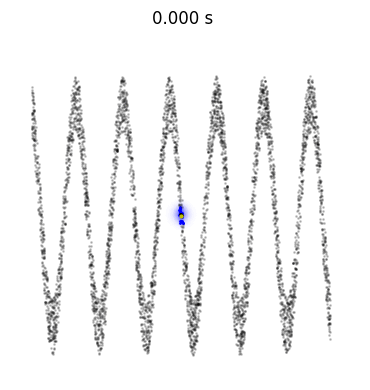
\includegraphics[width=0.49\textwidth]{simulation/5/frame_0.png}\hfill
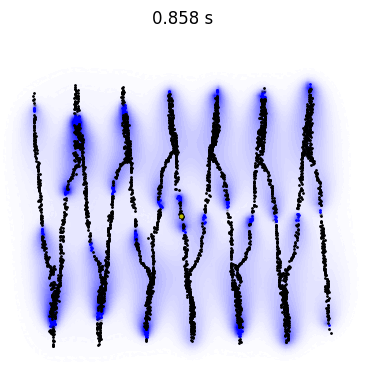
\includegraphics[width=0.49\textwidth]{simulation/5/frame_143.png}
\\[\smallskipamount]
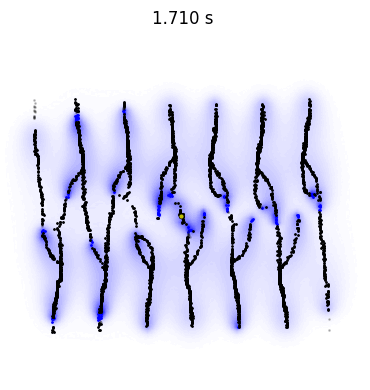
\includegraphics[width=0.49\textwidth]{simulation/5/frame_285.png}\hfill
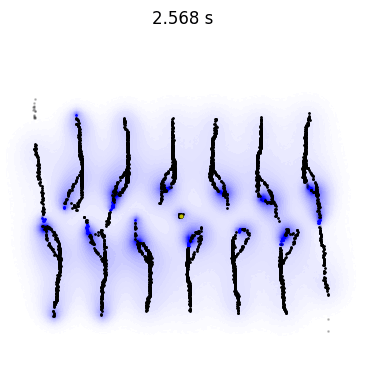
\includegraphics[width=0.49\textwidth]{simulation/5/frame_428.png}
\\[\smallskipamount]
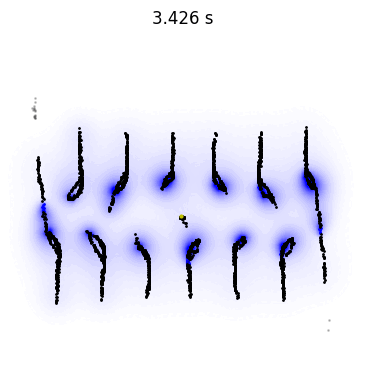
\includegraphics[width=0.49\textwidth]{simulation/5/frame_571.png}\hfill
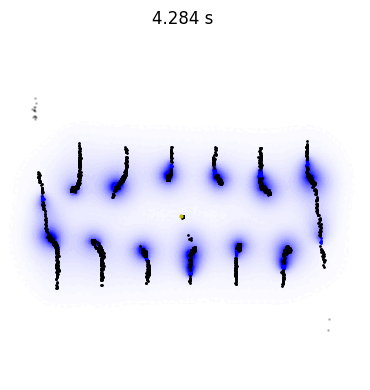
\includegraphics[width=0.49\textwidth]{simulation/5/frame_714.png}
\\[\smallskipamount]
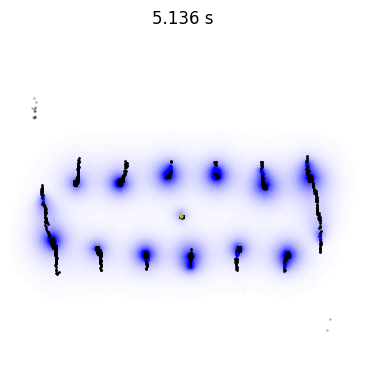
\includegraphics[width=0.49\textwidth]{simulation/5/frame_856.png}\hfill
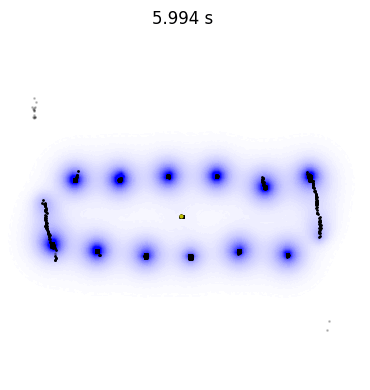
\includegraphics[width=0.49\textwidth]{simulation/5/frame_999.png}
\end{align*}
\end{minipage}
\begin{minipage}{0.45\textwidth}
\subsection{Sine Wave}
Here we used a distribution that resembles a sine curve to see how the chemical gets around sharper edges.
It appears that the particle chain breaks if there is a sharp turn involved.
We end up with \lq{}self-powered\rq{} blobs corresponding to the extrema of the sine wave.
\end{minipage}